%% Chapter: Modelado de Sistemas

\chapter{Modelado de Sistemas}

El Modelado de Sistemas es una actividad esencial de Ingeniería de Sistemas y de cualquier pensador sistémico. Pues, se hacen modelos como simplificación abstracta de la realidad \cite{Meadows-2009} que forma una representación del sistema real \cite{Fiuba-2005} o sistema origen a estudiar.

\section{Sistema de modelado}

Para entender la realidad se hace necesario percibirla y modelarla de algún modo. En este proceso existe un orden real de las cosas y un orden percibido y reflejado en un modelo hecho por alguien, un observador. Como dice Capra “toda la percepción de un modelo es, de alguna manera, la percepción de algún orden” \cite{Fritjof-Capra-1975} y la percepción de un orden es hecha por alguien. Un principio cibérnetico dice que todo fenómeno observado es observado por alguien (Heinz Von Foerster, 1979) que en otras palabras quiere decir que “todo conocer depende de la estructura del que conoce” \cite{Maturana-1984}. Por este motivo, en el sistema de modelado existe el observador como un elemento principal del mismo. Pero, además, para que el modelo resultado tenga alguna consistencia con la realidad modelada son necesarios conocimientos científico-técnicos que nos permitan cierta fiabilidad y herramientas conceptales y físicas para realizar dicha tarea.

\section{Herramientas conceptuales de modelado}

\subsection{Herramientas conceptuales de Diagramado}


\begin{table}[h]
\centering
\caption{Herramientas conceptuales de Diagramado}
\label{Herramientas-conceptuales-de-Diagramado}
\begin{tabular}{|l|l|}
\hline
Acrónimo & Significado en inglés                         \\ \hline
ADL      & Architecture Description Language             \\ \hline
BPMN     & Business Process Modeling Notation            \\ \hline
CD       & Conceptual Diagram or ConceptDraw             \\ \hline
CLD      & Causal Loop Diagram                           \\ \hline
ERD      & Entity Relationship Diagram                   \\ \hline
FC       & Flow Charts (for control flow)                \\ \hline
DFD      & Data Flow Diagram                             \\ \hline
MMD      & Map Mind Diagram                              \\ \hline
SC       & Structure Chart                               \\ \hline
SFD      & Stock and Flow Diagrams                       \\ \hline
SSADM    & Structured Systems Analysis and Design Method \\ \hline
UML      & Unified Modeling Language                     \\ \hline
\end{tabular}
\end{table}

\subsubsection{ADL}
\subsubsection{BPMN}
\subsubsection{CD}
\subsubsection{CLD}
\subsubsection{ERD}
\subsubsection{FC}
El Diagrama de Flujo (Flow Charts) es usado para diagramar flujos de control.

\subsubsection{DFD}

El Diagrama de Flujo de Datos o DFD fue introducido y popularizado en 1970 para el análisis y diseño estructurado \cite{Gane-Sarson-1979} para diagramar procesos de sistemas. Un DFD muestran el flujo de datos dentro del sistema desde entidades externas, mostrando como los datos fluyen entre diferentes procesos y qué almacenes intervienen para que los datos sean guardados y recuperados \cite{Scott-Ambler-2004}. 
Para este tipo de diagramas hay dos estándares de notaciones: la notación DeMarco-Yourdon (DeMarco, Yourdon y Constantine 1979 \cite{Dixit-2007}) y la notación Gane-Sarson.\newline
\newline
En este tipo de diagramas hay solo cuatro elementos \cite{Dixit-2007}:
\begin{itemize}
\item \textbf{Entidad externa:} son fuentes externas. En ambas notaciones se representa con cuadrados.
\item \textbf{Proceso:} son los subsistemas o procesos del sistema. En notación Gane-Sarson se representa con rectángulos redondeados y según DeMarco-Yourdon con círculos o elipses.  
\item \textbf{Flujo de dato:} flujo de datos electrónicos o físicos. En ambas notaciones se representa con flechas.
\item \textbf{Almacen:} almacen de información. En notación Gane-Sarson se representa con rectángulos abiertos y según DeMarco-Yourdon con rectangulos sin líneas laterales. Por practicidad se puede implementar con un rectángulo con algún distintivo, siempre cuando se aclare que la notación representa un almacen de datos.
\end{itemize}

\begin{figure}[h]
  \centering
  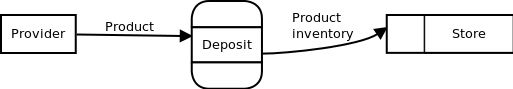
\includegraphics[scale=0.5]{DFDGaneSarsonNotation}
  \caption{DFD Notación Gane-Sarson \cite{Gane-Sarson-1979}}
  \centering
  \label{fig:DFDGaneSarsonNotation} %\ref{fig:DFDGaneSarsonNotation}
\end{figure}

\begin{figure}[h]
  \centering
  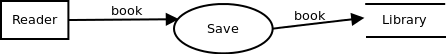
\includegraphics[scale=0.5]{DFDDeMarcoYourdonNotation}
  \caption{DFD Notación DeMarco-Yourdon \cite{Dixit-2007}}
  \centering
  \label{fig:DFDDeMarcoYourdonNotation} %\ref{fig:DFDDeMarcoYourdonNotation}
\end{figure}


\subsubsection{MMD}
\subsubsection{SC}
\subsubsection{SFD}
\subsubsection{SSADM}
\subsubsection{UML}

\section{Modelos de un sistema general}
\section{Sistema general de modelado}
\section{Modelo de sistemas generales básicos}
\subsection{Sistemas termodinámicos}
\subsection{Sistema aislado en equilibrio termodinámico}
\subsection{Sistema aislado tendiente al equilibrio}
\subsection{Sistema abierto en equilibrio estacionario}
\subsection{Sistema Sistemas en Equilibrio Dinámico}
\subsection{Sistemas Sostenibles y Sostenibilidad}
\subsection{Sistema Mínimo de Vida}
\subsection{Sistema Agente}
\subsection{Sistema Autopoiético Mínimo}
\section{Modelos de Sistemas Cibernético}

\subsection{Sistema Cibernético General}
\subsubsection{Ejemplo 1: Sistema regulador de tanque de agua}
\subsubsection{Ejemplo 2: Sistema regulador de Watt}
\subsubsection{Sistema Cibernético Auto-Aprendiente}
\subsubsection{Sistema Cibernético Auto-Organizado}
\subsubsection{Sistema Cibernético Auto-Aprendiz y Auto-Organizado}

\subsection{Modelos de organizaciones}
\subsubsection{Viable System Model}
